% Options for packages loaded elsewhere
\PassOptionsToPackage{unicode}{hyperref}
\PassOptionsToPackage{hyphens}{url}
\PassOptionsToPackage{dvipsnames,svgnames,x11names}{xcolor}
%
\documentclass[
  letterpaper,
  DIV=11,
  numbers=noendperiod]{scrartcl}

\usepackage{amsmath,amssymb}
\usepackage{iftex}
\ifPDFTeX
  \usepackage[T1]{fontenc}
  \usepackage[utf8]{inputenc}
  \usepackage{textcomp} % provide euro and other symbols
\else % if luatex or xetex
  \usepackage{unicode-math}
  \defaultfontfeatures{Scale=MatchLowercase}
  \defaultfontfeatures[\rmfamily]{Ligatures=TeX,Scale=1}
\fi
\usepackage{lmodern}
\ifPDFTeX\else  
    % xetex/luatex font selection
\fi
% Use upquote if available, for straight quotes in verbatim environments
\IfFileExists{upquote.sty}{\usepackage{upquote}}{}
\IfFileExists{microtype.sty}{% use microtype if available
  \usepackage[]{microtype}
  \UseMicrotypeSet[protrusion]{basicmath} % disable protrusion for tt fonts
}{}
\makeatletter
\@ifundefined{KOMAClassName}{% if non-KOMA class
  \IfFileExists{parskip.sty}{%
    \usepackage{parskip}
  }{% else
    \setlength{\parindent}{0pt}
    \setlength{\parskip}{6pt plus 2pt minus 1pt}}
}{% if KOMA class
  \KOMAoptions{parskip=half}}
\makeatother
\usepackage{xcolor}
\setlength{\emergencystretch}{3em} % prevent overfull lines
\setcounter{secnumdepth}{-\maxdimen} % remove section numbering
% Make \paragraph and \subparagraph free-standing
\ifx\paragraph\undefined\else
  \let\oldparagraph\paragraph
  \renewcommand{\paragraph}[1]{\oldparagraph{#1}\mbox{}}
\fi
\ifx\subparagraph\undefined\else
  \let\oldsubparagraph\subparagraph
  \renewcommand{\subparagraph}[1]{\oldsubparagraph{#1}\mbox{}}
\fi


\providecommand{\tightlist}{%
  \setlength{\itemsep}{0pt}\setlength{\parskip}{0pt}}\usepackage{longtable,booktabs,array}
\usepackage{calc} % for calculating minipage widths
% Correct order of tables after \paragraph or \subparagraph
\usepackage{etoolbox}
\makeatletter
\patchcmd\longtable{\par}{\if@noskipsec\mbox{}\fi\par}{}{}
\makeatother
% Allow footnotes in longtable head/foot
\IfFileExists{footnotehyper.sty}{\usepackage{footnotehyper}}{\usepackage{footnote}}
\makesavenoteenv{longtable}
\usepackage{graphicx}
\makeatletter
\def\maxwidth{\ifdim\Gin@nat@width>\linewidth\linewidth\else\Gin@nat@width\fi}
\def\maxheight{\ifdim\Gin@nat@height>\textheight\textheight\else\Gin@nat@height\fi}
\makeatother
% Scale images if necessary, so that they will not overflow the page
% margins by default, and it is still possible to overwrite the defaults
% using explicit options in \includegraphics[width, height, ...]{}
\setkeys{Gin}{width=\maxwidth,height=\maxheight,keepaspectratio}
% Set default figure placement to htbp
\makeatletter
\def\fps@figure{htbp}
\makeatother

\KOMAoption{captions}{tableheading}
\makeatletter
\makeatother
\makeatletter
\makeatother
\makeatletter
\@ifpackageloaded{caption}{}{\usepackage{caption}}
\AtBeginDocument{%
\ifdefined\contentsname
  \renewcommand*\contentsname{Table of contents}
\else
  \newcommand\contentsname{Table of contents}
\fi
\ifdefined\listfigurename
  \renewcommand*\listfigurename{List of Figures}
\else
  \newcommand\listfigurename{List of Figures}
\fi
\ifdefined\listtablename
  \renewcommand*\listtablename{List of Tables}
\else
  \newcommand\listtablename{List of Tables}
\fi
\ifdefined\figurename
  \renewcommand*\figurename{Figure}
\else
  \newcommand\figurename{Figure}
\fi
\ifdefined\tablename
  \renewcommand*\tablename{Table}
\else
  \newcommand\tablename{Table}
\fi
}
\@ifpackageloaded{float}{}{\usepackage{float}}
\floatstyle{ruled}
\@ifundefined{c@chapter}{\newfloat{codelisting}{h}{lop}}{\newfloat{codelisting}{h}{lop}[chapter]}
\floatname{codelisting}{Listing}
\newcommand*\listoflistings{\listof{codelisting}{List of Listings}}
\makeatother
\makeatletter
\@ifpackageloaded{caption}{}{\usepackage{caption}}
\@ifpackageloaded{subcaption}{}{\usepackage{subcaption}}
\makeatother
\makeatletter
\@ifpackageloaded{tcolorbox}{}{\usepackage[skins,breakable]{tcolorbox}}
\makeatother
\makeatletter
\@ifundefined{shadecolor}{\definecolor{shadecolor}{rgb}{.97, .97, .97}}
\makeatother
\makeatletter
\makeatother
\makeatletter
\makeatother
\ifLuaTeX
  \usepackage{selnolig}  % disable illegal ligatures
\fi
\IfFileExists{bookmark.sty}{\usepackage{bookmark}}{\usepackage{hyperref}}
\IfFileExists{xurl.sty}{\usepackage{xurl}}{} % add URL line breaks if available
\urlstyle{same} % disable monospaced font for URLs
\hypersetup{
  pdftitle={IMPACT OF ERRONEOUS DATA TRANSFORMATIONS ON ANALYSIS},
  pdfauthor={Junwei Chen},
  colorlinks=true,
  linkcolor={blue},
  filecolor={Maroon},
  citecolor={Blue},
  urlcolor={Blue},
  pdfcreator={LaTeX via pandoc}}

\title{IMPACT OF ERRONEOUS DATA TRANSFORMATIONS ON ANALYSIS}
\author{Junwei Chen}
\date{2024-02-24}

\begin{document}
\maketitle
\ifdefined\Shaded\renewenvironment{Shaded}{\begin{tcolorbox}[enhanced, sharp corners, interior hidden, borderline west={3pt}{0pt}{shadecolor}, breakable, boxrule=0pt, frame hidden]}{\end{tcolorbox}}\fi

\hypertarget{introduction}{%
\subsection{Introduction}\label{introduction}}

In this exercise we will generate some data from the normal distribution
with mean 1 and standard deviation 1. We then transform the data as
outlined in the \textbf{Data Simulation} section and proceed to
investigate whether the mean of the true data generating process is
greater than 0. We will then discuss some of the issues brought about by
the data transformations and what steps we can put in place to flag some
these issues during data analysis.

All the code for this exercise can be accessed at this link
\url{https://github.com/JunweiChen1012/Linear_models_tutorial}.

\hypertarget{data-simulation}{%
\subsection{Data Simulation}\label{data-simulation}}

We draw 1000 observations of data from the normal distribution of mean 1
and standard deviation 1. The last 100 observations are similar to the
first 100 observations. We then change half of the negative draws to
positive. Finally, we divide all observations with values between 1 and
1.1 by 10. The code that generates the observations can be accessed at
the link provided above.

\hypertarget{investigating-whether-the-mean-of-the-true-data-generating-process-is-greater-than-0}{%
\subsection{Investigating whether the mean of the true data generating
process is greater than
0}\label{investigating-whether-the-mean-of-the-true-data-generating-process-is-greater-than-0}}

To investigate whether the mean of the true data generating process is
greater than 0, we will use the one-sample t-test.

We can use the one-sample t-test because we have a large sample size of
1000 observations. Furthermore, a visual inspection of the histogram
plot of the sample data shows a bell-shape curve. This suggests
normality. See the histogram plot below.

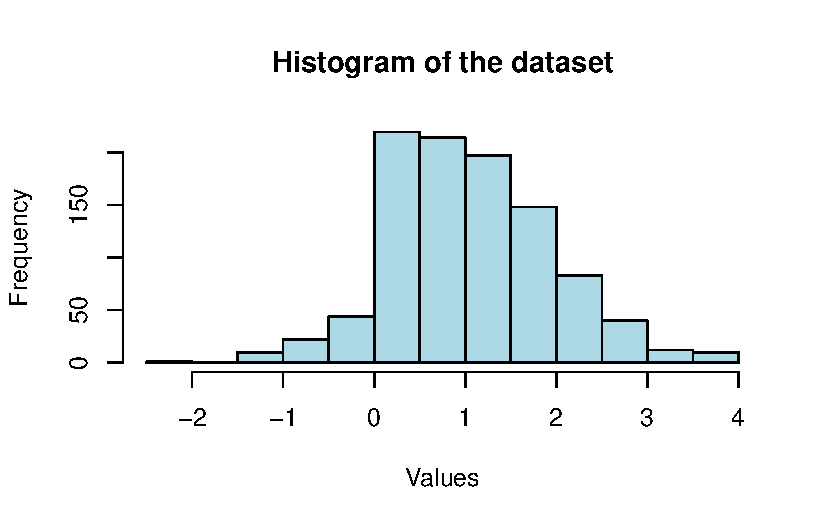
\includegraphics{report_files/figure-pdf/unnamed-chunk-2-1.pdf}

\hypertarget{one-sample-t-test}{%
\paragraph{One-sample t-test}\label{one-sample-t-test}}

Null hypothesis: true mean \textless= 0

Alternative hypothesis: true mean \textgreater{} 0

Below is the test result.

\begin{verbatim}

    One Sample t-test

data:  combined_sample_1000
t = 36.822, df = 999, p-value < 2.2e-16
alternative hypothesis: true mean is greater than 0
95 percent confidence interval:
 1.0117    Inf
sample estimates:
mean of x 
 1.059053 
\end{verbatim}

It can be observed that the p-value is less than our chosen significance
level (0.05), the test statistic is positive and the confidence interval
for the mean does not include 0. These observations give sufficient
evidence to suggest that the true mean of the data generating process is
greater than 0.

\hypertarget{issues-brought-about-by-the-data-transformations}{%
\subsection{Issues brought about by the data
transformations}\label{issues-brought-about-by-the-data-transformations}}

In order to investigate the impact of the data transformations, we will
compute summary statistics (median, mean, and standard deviation) of the
relevant datasets before and after each transformation to assess the
impact of the data transformations.

We will then proceed to plot a histogram of each of the datasets to
determine whether a visual inspection of the plots would have been
useful in flagging the unintended data transformations.

Below is a description of each of the datasets whose summary statistics
will be computed.

\hypertarget{datasets}{%
\paragraph{Datasets}\label{datasets}}

\textbf{original} - 1000 observations drawn from the normal distribution
with a mean of 1 and standard deviation of 1.

\textbf{duplicates} - a derivative of the \texttt{original} dataset
above. However, the last 100 values have been replaced with the first
100 values.

\textbf{half\_neg\_to\_pos} - a derivative of the \texttt{duplicates}
dataset above. However, half the negative values were then converted
into positive values.

\textbf{div\_by\_10} - a derivative of the \texttt{half\_neg\_to\_pos}
dataset above. However all values between 1 and 1.1 were divided by 10.

\hypertarget{summary-statistics}{%
\paragraph{Summary statistics}\label{summary-statistics}}

Below are the generated summary statistics.

\begin{verbatim}
                   Median      Mean        SD
Original        1.0196749 1.0108092 0.9879296
Duplicates      1.0138680 0.9949568 0.9953398
Half_neg_to_pos 1.0647365 1.0864445 0.8944764
Div_by_10       0.9777297 1.0590530 0.9095233
\end{verbatim}

It can be observed that each transformation of the dataset had an impact
on the mean, median and standard deviation. As a result of this, it is
recommended to compute and monitor the dataset summary statistics as
part of the data analysis process.

\hypertarget{visual-inspection-of-plots}{%
\paragraph{Visual Inspection of
Plots}\label{visual-inspection-of-plots}}

Below are the histograms of the 4 datasets. The impact of the unintended
data transformations are visible in the plots.

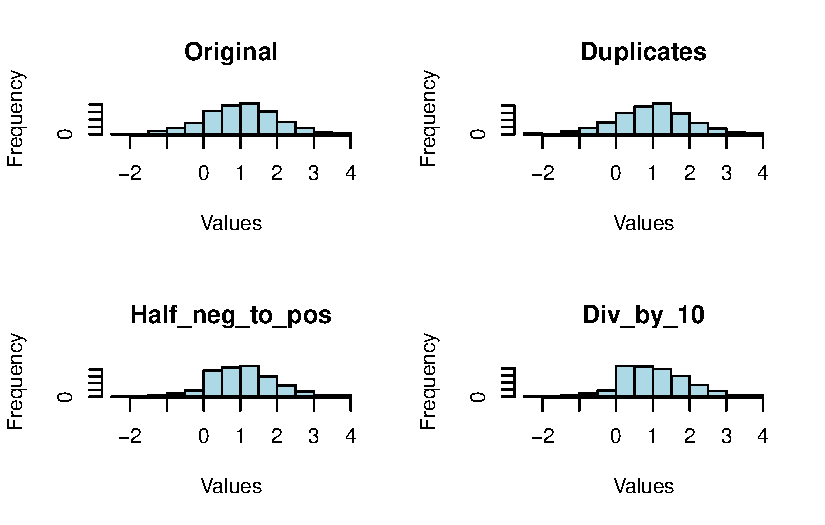
\includegraphics{report_files/figure-pdf/unnamed-chunk-6-1.pdf}

Let us review the plots one by one. When we compare \texttt{duplicates}
against \texttt{original}, there is not much of a difference in the
plots so we are not able to flag the impact of duplicating the first 100
observations in the dataset.

However, comparing \texttt{Half\_neg\_to\_pos} histogram against
\texttt{Duplicates} and \texttt{Original} histograms we note that the
frequency of values less than 0 has decreased. This should prompt us to
investigate what happened. When we check the data, we note that
initially, there were 153 negative values in the \texttt{duplicates}
dataset however only 77 negative values remained in the
\texttt{half\_neg\_to\_pos} dataset.

When we compare the \texttt{Div\_by\_10} histogram to the other
histograms, we notice that the frequency of values between 0 and 1.5 has
changed. For example, in the \texttt{Half\_neg\_to\_pos} histogram, the
frequency of values between 0 and 1.5 seems to be increasing at each
step however in the \texttt{Div\_by\_10} histogram, the frequency is
decreasing. This should prompt an investigation to find out what
happened.

Therefore, it is recommended to plot and visually examine data plots as
part of the data analysis process to flag any errors that might arise.



\end{document}
